% 
% chapter3.tex
% ThesisISEL
% 
% Created by Serge Lage on 2019/07/30.
%
% ================
% = Data =
% ================
\chapter{Data Analysis}
\label{cha:data}
This chapter provides information on data and analysis methodologies.



\section{VMS Records} % (fold)
\label{sec:vms_records}

VMS Data provided by the Xsealence \cite{WEBSITE:Xsealence} enterprise contained data generated by the MONICAP \cite{WEBSITE:MonicapXsealence} "Blue Box". Information about the localization, direction, and velocity of the vessel, every 10 minutes is saved in a local database. VMS datasets contained a vessel identification code, a timestamp, the latitude and longitude positions, the speed and the direction. In this dataset, there are 769930 entries from thirty-eight vessels, between 2008-10-30 and 2016-11-04. These data are from vessels operating in the Portuguese shore. 
This dataset is created automatically by the MONICAP system and follows the concept of integrity and confidentiality.\\
The variables registered in the dataset are:
\begin{itemize}
\item VesselID: Vessel identification;
\item Utc: Date time of the log;
\item Gps-id: identification of the GPS in use (0 = GPS with EGNOS, 1 = MiniCs GPS);
\item Fix/fix2: types of fix in the GPS:
\begin{itemize}
\item 0 = invalid, 
\item 1 = standard: valid, without integrity (without EGNOS), 
\item 2 = differential: valid, with integrity (with EGNOS), 
\item 3 = integrity: valid with integrity (with EGNOS);
\end{itemize}
\item Lat/Lat2: latitude of GPS primary/secondary (in decimal);
\item Lon/Lon2: longitude of GPS primary/secondary (in decimal);
\item Cog: Course Over Ground. Varies from 0 to 360 clockwise, being 0, facing north;
\item Sog: Speed Over Ground (velocity in knots);


\end{itemize}


In Table \ref{table:vms_records}, we can see the summary of the data used in this project. The number of occurrences is 769930. 
Some cells of the table are empty due to some measures that do not apply to qualitative data.
The P\textsubscript{25} stands for the 1\textsuperscript{st} Quartile, P\textsubscript{75} stands for the 3\textsuperscript{rd} Quartile and \textit{SD} stands for Standard deviation.

\begin {table}[h]
\small
\begin{center}
\begin{tabular}{c|c|c|c|c|c|c|c}
& Minimum & Maximum & Average & P\textsubscript{25} & Median & P\textsubscript{75} & SD\\
\hline
Lon & -52.706 & 35.965 & -4.493 &-9.811&-9.115&-7.986&21.156\\
Lat & -35.243 &76.064&25.933&33.038&38.423&40.21&25.916\\
Sog & 0 &42&4.183&1.634&3.012&7.399&3.211\\
Cog & 0&360&166.31&68.89&173.125&255.69&108.64\\
utc & 2008-10-30 & 2016-11-04 &-&-&-&-&-\\
gps\_ id & 0&1&-&-&-&-&-\\
fix & 1&3&-&-&-&-&-\\
Fix2 & 0&2&-&-&-&-&-\\
Lon2 & -52.706&155.977&-3.702&-9.726&-8.991&0&20.933\\
Lat2 & -35.24&76.064&23.663&0&37.595&40.191&26.383\\
VesselId & 1&38&-&-&-&-&-
\label{table:vms_records}
\end{tabular}
\caption {VMS Records}
\end{center}
\end {table}


% section vms_records (end)
\newpage 


\section{VMS Vessels} % (fold)
\label{sub:vms_vessels}
VMS Vessels data is the vessel information that goes along with the VMS Records. These data contain information about vessels and fishing activities for which they are licensed. This data is created by the competent authority that process fisheries licensing. \\
The variables registered in the dataset are:
\begin{itemize}
\item ID: Vessel identification (VesselID/VMSRecords, foreign key);
\item Name: Name of the vessel;
\item Loa: Length Overall; 
\item GT: Gross Tonnage;
\item HP: Vessel power (HP);
\item kW: Vessel power (KW);
\item License: Registration of the vessel's licenses;
\item PriGearCode: FOA code of the principal fishery device;
\item SecGearCode: FOA code of the secondary fishery device.
\end{itemize}
%In Appendix A a detailed descriptive analysis of these variables is provided.

In Table \ref{table:vms_vessels} we can see the summary of the data regarding the vessels in the table VMS Records. This data was filtered from 56 occurrences to 38. The deleted data was referred to Vessels that have not data in the table VMS Records, so this vessel information was superfluous to our needs. In Appendix \ref{appendix:anexo1} we discriminate the fishing licenses. 


\begin {table}[H]
\small
\begin{center}
\begin{tabular}{c|c|c|c|c|c|c|c}
& Minimum & Maximum & Average & P\textsubscript{25} & Median & P\textsubscript{75} & SD \\
\hline
ID & 1&38&-&-&-&-&-\\
Name &-&-&-&-&-&-&-\\
Loa & 11.95&84.94&23.48&16.93&19.35&23.70&15.49\\
GT &22251&18.99&200.28&27.98&57.15&110.34&473.78\\
HP & 3600&130&539&230&350&497&689.56\\
KW &2684.50&95.62&396.52&172.84&259.21&367.91&498.54\\
License &-&-&-&-&-&-&-\\
PriGC &-&-&-&-&-&-&-\\
SecGC &-&-&-&-&-&-&-


\label{table:vms_vessels}
\end{tabular}
\caption {VMS Vessels}
\end{center}
\end {table}

% section vms_vessels (end)


\section{Descriptive Data Analysis} % (fold)
\label{sub:data_analysis}



The data used as input to the models is VMS Records data. Among these data, those that bet distinguish between different types of fishing activity are speed and location.\\
About the locations, certain fishing types only occur in certain depth. So the locations can help in these cases. \\
To meet the objectives, we need to understand the velocity patterns.
By studying and analyzing the velocity data, it was possible to verify the existence of two velocity distributions.

\begin{figure}[h]
\centering
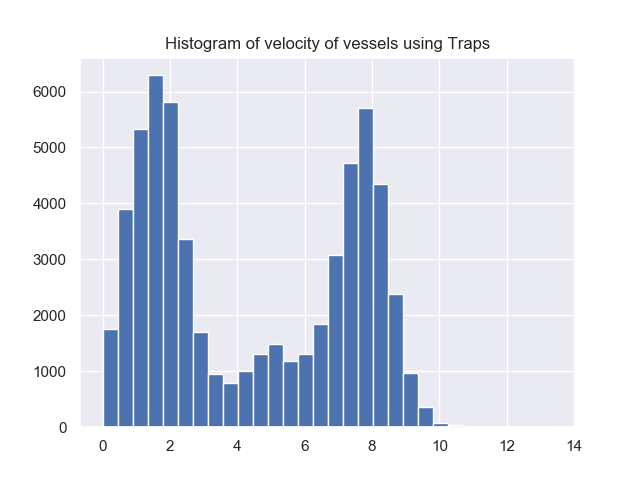
\includegraphics[width=0.8\linewidth]{Chapters/img/h_armadilhas.png}
\caption{Histogram of velocity of traps license.}
\label{fig:h_armadilhas}
\end{figure}

%\begin{figure}[h]
% \centering
% 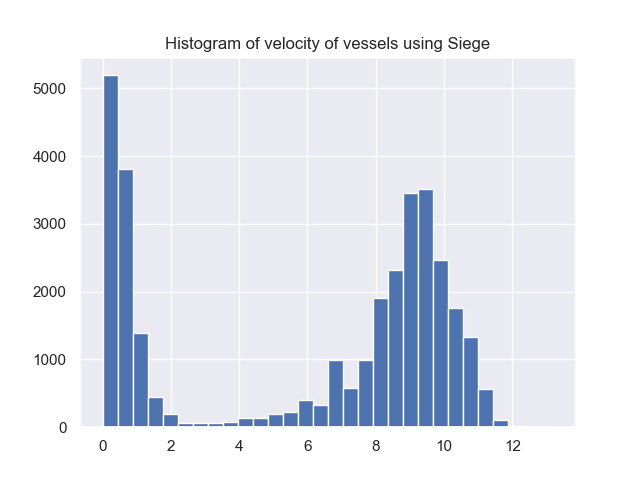
\includegraphics[width=0.8\linewidth]{Chapters/img/h_cerco.png}
% \caption{Histogram of velocity of siege license.}
% \label{fig:h_cerco}
%\end{figure}

\begin{figure}[h]
\centering
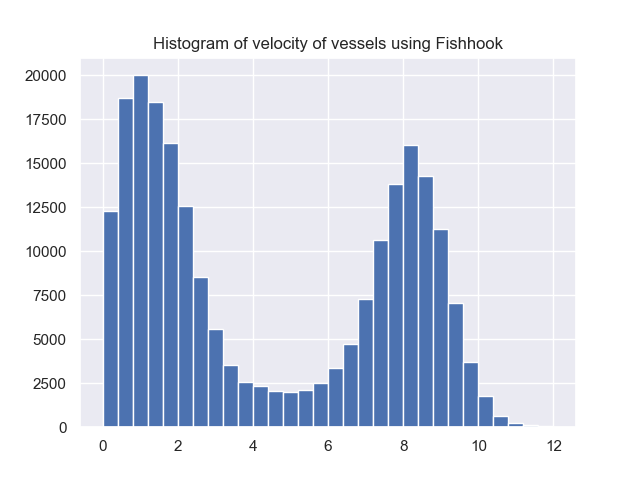
\includegraphics[width=0.8\linewidth]{Chapters/img/h_linha.png}
\caption{Histogram of velocity of fishhook license.}
\label{fig:h_linha}
\end{figure}

In Figure \ref{fig:h_armadilhas} it is possible to distinguish two different speed distributions, the lower speeds correspond to fishing activities, and the higher speeds represent the movements of the vessel from the port to the fishing grounds and back to the port \cite{MappingFishing}.





Knowing this, we can notice that different types of fishing have different fishing speeds, as we can see the differences between the histogram in Figure \ref{fig:h_armadilhas} containing data on fishing vessels using traps and Figure \ref{fig:h_linha} concerning fishing vessels using fishhook.





It is essential to separate the inputs representing fishing speeds from the others in the data as the input to the models used in Chapter 5 it is necessary to have the data filtered out only with the fishing activity data. This because we will only use the fishing speed to study and create the methodology's necessary to achieve the proposed goals.

Data from operations other than fisheries should be discarded as they do not discriminate against different types of fishing. For example, speed 0 nautical miles is not interesting regardless of their type of fishing, once all vessels stop in the fishing port.


% section data_analysis (end)

% chapter data (end)




